\chapter{Characterization of Components and Equipment}
\todo{add references to all datasheets of which specifiactions were taken}
\todo{add pictures}

\section{R\&S Vector Network Analyzer ZNB8}
In order to gain a deeper unserstanding of the non-idealities of the
components which were later used for the different test setups
were characterized using a Rohde \& Schwarz Vector Network Analyzer. \\

Besides the results of the measurements of which a few a presented
in the next few sections, also important lessons about measuring were
learned. It took me about one week to be able to performe meaningfull
measurements on the ZNB4 and to understand it's features.
While performing different measurements it soon became very clear then
non optimal torque while connection plugs or overbend cables
can produce notches of dozens of dBs even when using highest quality
equipment. \\

\begin{table}[h]
  \centering
  \begin{tabular}{|l|l|}
    \hline
    Frequency range & 9 kHz to 8.5 GHz \\ \hline
    Sweep speed & about 1ms for 100 points \\ \hline
    Dynamic range & up to 140 dB \\ \hline
    Power sweep range & 98 dB \\ \hline
  \end{tabular}
  \caption{Key properties of R\&S Vector Network Analyzer ZNB8}
  \label{tab:awg}
\end{table}

\section{Arbitrary waveform generator: Tektronix AWG 7122C}
\label{sec:comp_awg}

An \acrfull{AWG} was used instead of a real transmitter.
Not only because there is no transmitter available but also because of
it's flexibility. The same Matlab script used for simulations could
also call function output the baseband or the \gls{IF} signal.
The additional marker outputs could be used to trigger the oscilloscope
as well as the data acquisition process on the \gls{FPGA}.

\begin{table}[h]
  \centering
  \begin{tabular}{|l|l|}
    \hline
    Sample Rate & 12 $\text{GS}/\text{s}$, 24 $\text{GS}/\text{s}$ (interleaved) \\ \hline
    Number of analog channels & 2, 1 interleaved \\ \hline
    Analog bandwidth & 5.6 GHz \\ \hline
    Number of digital maker channels & $2 \times 2$ \\ \hline
    Vertical resoluation & 8 Bit, 10 Bit when markers are disabled \\ \hline
    Maximal waveform length & $\approx 130$ MS  \\ \hline
  \end{tabular}
  \caption{Key properties of Tektronix AWG 7122C}
  \label{tab:awg}
\end{table}

\section{Sivers IMA 58-63 GHz Converter FC1005V/00}
\label{sec:comp_sivers}
The most important is componant in the transmission chain is the
up- and downconverter from an \acrfull{IF} to the \acrfull{RF}.
For this purpose the Sivers IMA FC1005V/00 module was used.
It consists of an independent transmitt and receive path including
a horn antenna assembly, amplifiers, up-/downmixers and a pll
for frequency synthesis. It is able up-/downmix an \gls{IF}
of between 1 and 5 GHz to the \gls{RF} of 58 to 63 GHz. \\

As shown in \figref{fig:sivers} both the transmitt and receive path
use two inputs (I- and Q-channel) which are then both mixed to
\gls{RF} and than fed to a $90^\circ$ hybrid coupler. \\
This results in one of the two mirror frequency to be completely canceled
iff it of the two channel is shifted by $-90^\circ$ relative to the other.
This can be done by using another $90^\circ$ hybrid coupler working on
\gls{IF} as described in \secref{sec:comp_90deg} or by using die Hilbert
transform as shown in \todo{referenc to theory}. \\
The Sivers module is build such that it transmitts on the \gls{USBand}
(canceling the \gls{LSBand}) when the Q-channel is connected to the signal
$x(t)$ and the I-channel to $\mathcal{H}\{x(t)\}$.
\todo{describe how receiver has to be connected for LSB and double check it} \\

There are two inpepentend \gls{LO} for transmission and reception both using
the reference. There is an internal 10 MHz reference on the board. During
most measurements the reference was locked to same external reference as the
\gls{AWG} and \gls{ADC} to not have any frequency offsets when different
transmitt and receive frequencies were used.

\begin{figure}
  \centering
  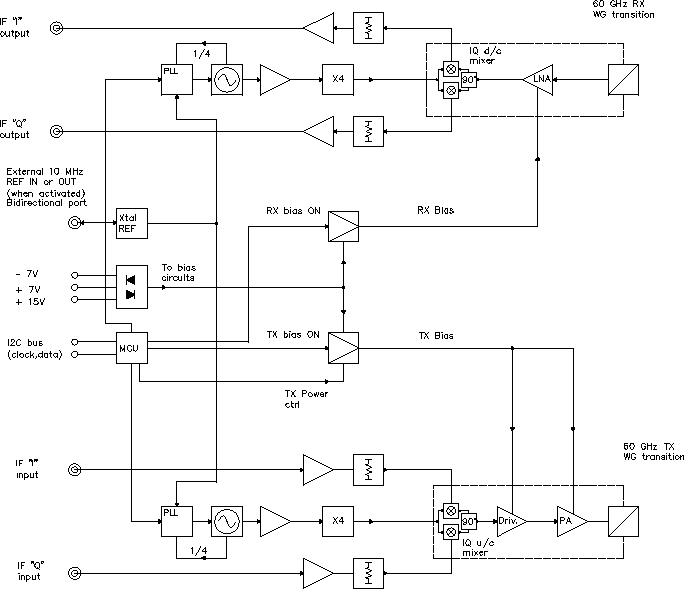
\includegraphics[width=\textwidth]{figures/sivers_block_diagram}
  \caption{Block diagram of Sivers IMA FC1005V/00 Converter}
  \label{fig:sivers}
\end{figure}
\todo{add reference to siversima}

\begin{table}[h]
  \centering
  \begin{tabular}{|l|l|}
    \hline
    \acrshort{TX} and \acrshort{RX} \gls{RF} range & 58 - 63 GHz \\ \hline
    \acrshort{TX} and \acrshort{RX} \gls{IF} range & 1 - 5 GHz \\ \hline
    Saturated output power & min 16 dBm \\ \hline
    \gls{LO} leakage & typical 10 dBm, max 15 dBm \\ \hline
    \acrshort{TX} Image rejection & min 10 dB, typical 20 dB \\ \hline
    \acrshort{RX} Image rejection & min 10 dB, typical 14 dB \\ \hline
    Total Power Consumption & 9.5 W \\ \hline
  \end{tabular}
  \caption{Key properties of 58-63 GHz V-band Converter Sivers IMA FC1005V/00}
  \label{tab:awg}
\end{table}

\section{Meca 3 dB Hybrid Coupler 705S-3.000}
\label{sec:comp_90deg}

A Hybrid coupler has typically 4 ports as shown on
\figref{fig:90deg_coupler_symbol}.
One port is often 50 $\Omega$ determinated and therefor might not be connected
to a plug. \\

It is when neglacting production imperfections a fully symetric component
(inputs $x_i(t)$ with outputs $y_i(t)$ as well as indices 1 and 2
can be exchanged) and has the following relations:

\[y_1(t) = \frac{1}{\sqrt{2}} \left[x_1(t) \angle -\frac{\pi}{2} + x_2(t) \angle -\pi \right] \]
\[y_2(t) = \frac{1}{\sqrt{2}} \left[x_1(t) \angle -\pi + x_2(t) \angle -\frac{\pi}{2} \right] \]

As shown in \figref{fig:90deg_coupler_measurement} the power of
$x_1$ is not perfect equally splitted to $y_1$ and $y_2$. The power difference
is smaller than 1 db in the band from 1.8 Ghz to 4 GHz.
Also there is a little power ($\leq -20 db$) leaking from $x_1$ to $x_2$ and from
$y_1$ to $y_2$. \\

Due to missing calibration equipment the phase rotation could not be measured.
All measured numbers matched the specifications.

\begin{figure}
  \centering
  
\includegraphics{figures/90deg_coupler_symbol}
  \caption{Symbol of a $90^\circ$ Coupler}
  \label{fig:90deg_coupler_symbol}
\end{figure}

\begin{figure}
  \centering
  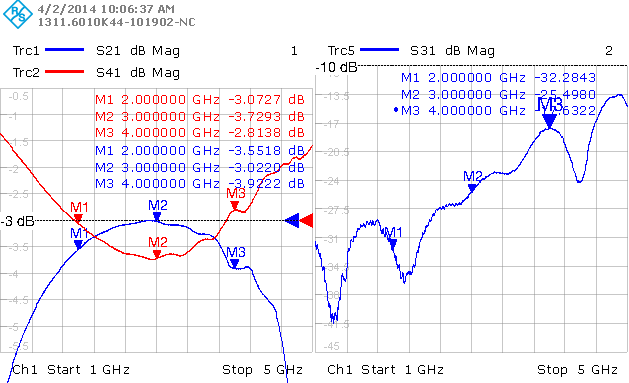
\includegraphics[width=\textwidth]{figures/Meca_705S-3_coupler_id1}
  \caption{Measurements of Meca 3 dB Hybrid Coupler 705S-3.000,
    $x_1 \triangleq $ port 1, $y_1 \triangleq $ = port 2,
    $x_2 \triangleq $ port 3, $y_2 \triangleq $ = port 4}
  \label{fig:90deg_coupler_measurement}
\end{figure}

\begin{table}[h]
  \centering
  \begin{tabular}{|l|l|}
    \hline
    Operation range & 2 - 4 GHz \\ \hline
    Frequency Sensitivity & $\pm$ 0.4 dB \\ \hline
    Coupling variation & 3.1 dB $\pm$ 0.6 db \\ \hline
    Typical Isolation & 22 dB \\ \hline
    max VSWR & 1.2 : 1 \\ \hline
    Phase rotation & $90^\circ \pm 2.0^\circ$ \\ \hline
  \end{tabular}
  \caption{Key properties of Meca 3 dB Hybrid Coupler 705S-3.000}
  \label{tab:awg}
\end{table}

\todo{add reference}
% http://e-meca.com/rf-directional-coupler/specs_hybrid.php?ID=23&SpecsID=22#

\section{Mini-Circuits: High-Pass Filter, Amplifiers}
\begin{itemize}
\item Table with most important features
\item Show measurements done with Network Analyzer
\end{itemize}

\section{Texas-Instruments Balun ADC-WB-BB}
\begin{itemize}
\item Table with most important features
\item Show measurements done with Network Analyzer
\end{itemize}

\section{Mini-Circuits DC Block MCL BLK-89-S+}
\label{sec:comp_dc_block}
To prevent \acrshort{DC} from driving amplifier inputs into saturation
a \acrshort{DC} block was used. A significatly higher insertion loss was
measured than specified in the data sheet as shown in
\figref{fig:comp_dc_block_insertion_loss}.

\begin{table}[h]
  \centering
  \begin{tabular}{|l|l|}
    \hline
    Pass Band & 0.1 MHz to 8 GHz \\ \hline
    Specified Insertion loss up to 4 GHz & < 0.8 dB \\ \hline
    Measured Insertion loss up to 4 GHz & < 0.8 dB \\ \hline
  \end{tabular}
  \caption{Key properties of Mini-Circuits DC Block MCL BLK-89-S+}
  \label{tab:awg}
\end{table}

\begin{figure}
  \centering
  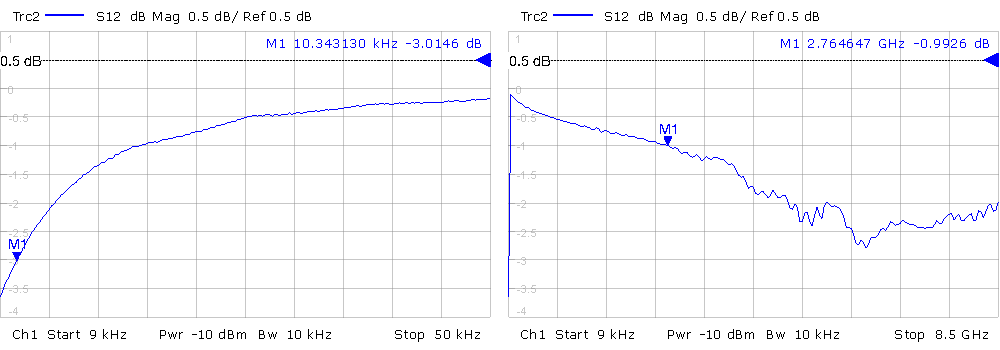
\includegraphics[width=\textwidth]{figures/MCL_BLK-89-S+_DC-Block_insertion_loss}
  \caption{Measured Insertion Loss of Mini-Circuits DC Block MCL BLK-89-S+}
  \label{fig:comp_dc_block_insertion_loss}
\end{figure}

\section{Texas Instruments ADC 12d1800}
\label{sec:comp_adc}
The receiver was build using the Ultra High-Speed ADC12D1800 by Texas Instruments.
It is able to either sample two channels at 1.8 $\text{GS}/\text{s}$ or to interleave
this two channels by applying the same input signal to both channels and sampling
one on the positive and the other one on the negative clock edge resulting in sample
rates of up to 3.6 $\text{GS}/\text{s}$. The vertical resolution of 12 bits is better
than the one of the used oscilloscope (\secref{sec:comp_osci}) and in most scenarios
not the \gls{SNR} limiting factor even when the signal is 6 db below full-scale.
The huge analog bandwidth of about 100 kHz
(limited by the \gls{DC} block described in \secref{sec:comp_dc_block}) to about
2.8 GHz allows to not only sample the first Nyquist zone but also allows
for sub-sampling which was particular interest. \\

The ADC12D1800 Reference Board was used which has a very well optimized board
layout, supports SMA plugs for all important signals, includes a \gls{FPGA}
and \gls{USB} interface for configuration and a power supply. The reference
board has an onboard \gls{PLL} but was often clocked by a marker output of the
\gls{AWG}. An \gls{FMC} connector exposes the full interface of the \gls{ADC} to
the on board \gls{FPGA} and is used by the Virtex-7 board to capture the data
as described in \chapref{chap:fpga}. \\

\begin{table}[h]
  \centering
  \begin{tabular}{|l|l|}
    \hline
    Number of channels & 2, 1 interleaved \\ \hline
    Sample Rate & $\leq$ 1.8 $\text{GS}/\text{s}$, $\leq$ 3.6 $\text{GS}/\text{s}$ interleaved \\ \hline
    Analog Bandwidth & typical 2.8 GHz \\ \hline
    Vertical Resolution & 12 bit \\ \hline
    Noise Floor Density & $\approx$ -150 $\text{dB}/\text{Hz}$ \\ \hline
    Power Consumption & 4.7 W \\ \hline
  \end{tabular}
  \caption{Key properties of Texes-Instruments ADC 12d1800}
  \label{tab:awg}
\end{table}

\section{Xilinix Virtex 7 Board VC707}
\label{sec:comp_virtex7}
\begin{itemize}
\item Table with most important features
\end{itemize}

\section{R\&S Oscilloscope RTO 1044}
\label{sec:comp_osci}
High frequency measurements were made on a Rohde \& Schwarz Digital
Oscolloscope RTO 1044. With the optional reference input it could be locked
to the \gls{AWG} as well used to have a very precise ($\pm 0.02 \text{ppm}$),
oven controlled 10 MHz reference. \\

During many experiments the real time \gls{FFT} display of the oscilloscope was
proven very usefull to check power levels and signal shapes. \\

Since the VISA standard for instrument control is painfull to install under
Redhat 6 a small programm based on the VXI-11 library written by
Steve D. Sharples \todo{reference: http://optics.eee.nottingham.ac.uk/vxi11/}
was written to convert sinmple telnet commands send by Matlab
to remote procedure calls. This allowed to setup and readout the oscilloscope
directly in the Matlab simulation framework. This was used to do first experiments
on the actual \gls{RF} hardware before the \gls{FPGA} (\chapref{chap:fpga}) was
completely implemented. \\

\begin{table}[h]
  \centering
  \begin{tabular}{|l|l|}
    \hline
    Number of channels & 4, 2 interleaved \\ \hline
    Sample Rate & 10 $\text{GS}/\text{s}$, 20 $\text{GS}/\text{s}$ interleaved \\ \hline
    Analog Bandwidth at 50 $\Omega$ & $\geq 4$ Ghz \\ \hline
    Vertical Resolution & 8 bit \\ \hline
  \end{tabular}
  \caption{Key properties of R\&S Oscilloscope RTO 1044}
  \label{tab:awg}
\end{table}
